% Options for packages loaded elsewhere
\PassOptionsToPackage{unicode}{hyperref}
\PassOptionsToPackage{hyphens}{url}
%
\documentclass[
]{article}
\usepackage{amsmath,amssymb}
\usepackage{lmodern}
\usepackage{iftex}
\ifPDFTeX
  \usepackage[T1]{fontenc}
  \usepackage[utf8]{inputenc}
  \usepackage{textcomp} % provide euro and other symbols
\else % if luatex or xetex
  \usepackage{unicode-math}
  \defaultfontfeatures{Scale=MatchLowercase}
  \defaultfontfeatures[\rmfamily]{Ligatures=TeX,Scale=1}
\fi
% Use upquote if available, for straight quotes in verbatim environments
\IfFileExists{upquote.sty}{\usepackage{upquote}}{}
\IfFileExists{microtype.sty}{% use microtype if available
  \usepackage[]{microtype}
  \UseMicrotypeSet[protrusion]{basicmath} % disable protrusion for tt fonts
}{}
\makeatletter
\@ifundefined{KOMAClassName}{% if non-KOMA class
  \IfFileExists{parskip.sty}{%
    \usepackage{parskip}
  }{% else
    \setlength{\parindent}{0pt}
    \setlength{\parskip}{6pt plus 2pt minus 1pt}}
}{% if KOMA class
  \KOMAoptions{parskip=half}}
\makeatother
\usepackage{xcolor}
\IfFileExists{xurl.sty}{\usepackage{xurl}}{} % add URL line breaks if available
\IfFileExists{bookmark.sty}{\usepackage{bookmark}}{\usepackage{hyperref}}
\hypersetup{
  hidelinks,
  pdfcreator={LaTeX via pandoc}}
\urlstyle{same} % disable monospaced font for URLs
\usepackage[left=1cm,right=1cm,top=1.8cm,bottom=1.0cm]{geometry}
\usepackage{graphicx}
\makeatletter
\def\maxwidth{\ifdim\Gin@nat@width>\linewidth\linewidth\else\Gin@nat@width\fi}
\def\maxheight{\ifdim\Gin@nat@height>\textheight\textheight\else\Gin@nat@height\fi}
\makeatother
% Scale images if necessary, so that they will not overflow the page
% margins by default, and it is still possible to overwrite the defaults
% using explicit options in \includegraphics[width, height, ...]{}
\setkeys{Gin}{width=\maxwidth,height=\maxheight,keepaspectratio}
% Set default figure placement to htbp
\makeatletter
\def\fps@figure{htbp}
\makeatother
\setlength{\emergencystretch}{3em} % prevent overfull lines
\providecommand{\tightlist}{%
  \setlength{\itemsep}{0pt}\setlength{\parskip}{0pt}}
\setcounter{secnumdepth}{-\maxdimen} % remove section numbering
\usepackage{fancyhdr} \pagestyle{fancy} \usepackage{graphicx} \usepackage{eurosym} \usepackage{xcolor} \usepackage{booktabs,xcolor} \usepackage{setspace} \definecolor{myblue}{HTML}{5F7ED9} \definecolor{wblight}{HTML}{f8f4fc} \definecolor{wbmid}{HTML}{f0ecfc} \definecolor{wbpurple}{HTML}{c8c4ec} \definecolor{wbfemale}{HTML}{303c84} \definecolor{wbmale}{HTML}{707cbc} \rfoot{\mbox{\kern\dimexpr-1cm
\includegraphics[width=\paperwidth]{footer.png}}} \fancypagestyle{plain}{\pagestyle{fancy}} \pagenumbering{gobble} \usepackage[defaultfam,tabular,lining]{montserrat} \usepackage[fontsize=8pt]{scrextend} \usepackage{float} \restylefloat{table} \usepackage{multicol} \usepackage{paralist} \usepackage{hyperref} \newcommand{\hideFromPandoc}[1]{#1} \hideFromPandoc{ \let\Begin\begin \let\End\end } \usepackage{caption} \usepackage[framemethod=tikz]{mdframed} \newmdenv[innerlinewidth=0.5pt, roundcorner=24pt,linecolor=white,backgroundcolor=wbpurple,innerleftmargin=2pt,innerrightmargin=2pt,innertopmargin=2pt,innerbottommargin=0pt,nobreak=True,leftmargin = 3.5pt,rightmargin = 3.5pt]{mybox} \newcommand*\circled[1]{\tikz[baseline=(char.base)]{ \node[shape=circle,text width=30pt,align=center,draw=wbpurple,minimum size=30pt,outer sep=0pt,fill=wblight] (char) {#1};}} \newcommand*\squared[1]{\tikz[baseline=(char.base)]{ \node[shape=rectangle,text width=3.15cm,align=center,draw=wbpurple,minimum size=1.5cm,outer sep=0pt,inner sep=4pt,fill=wblight] (char) {#1};}} \captionsetup{skip=0pt} \setlength{\headsep}{.5cm}
\usepackage{booktabs}
\usepackage{longtable}
\usepackage{array}
\usepackage{multirow}
\usepackage{wrapfig}
\usepackage{float}
\usepackage{colortbl}
\usepackage{pdflscape}
\usepackage{tabu}
\usepackage{threeparttable}
\usepackage{threeparttablex}
\usepackage[normalem]{ulem}
\usepackage{makecell}
\usepackage{xcolor}
\ifLuaTeX
  \usepackage{selnolig}  % disable illegal ligatures
\fi

\author{}
\date{\vspace{-2.5em}}

\begin{document}

\lhead{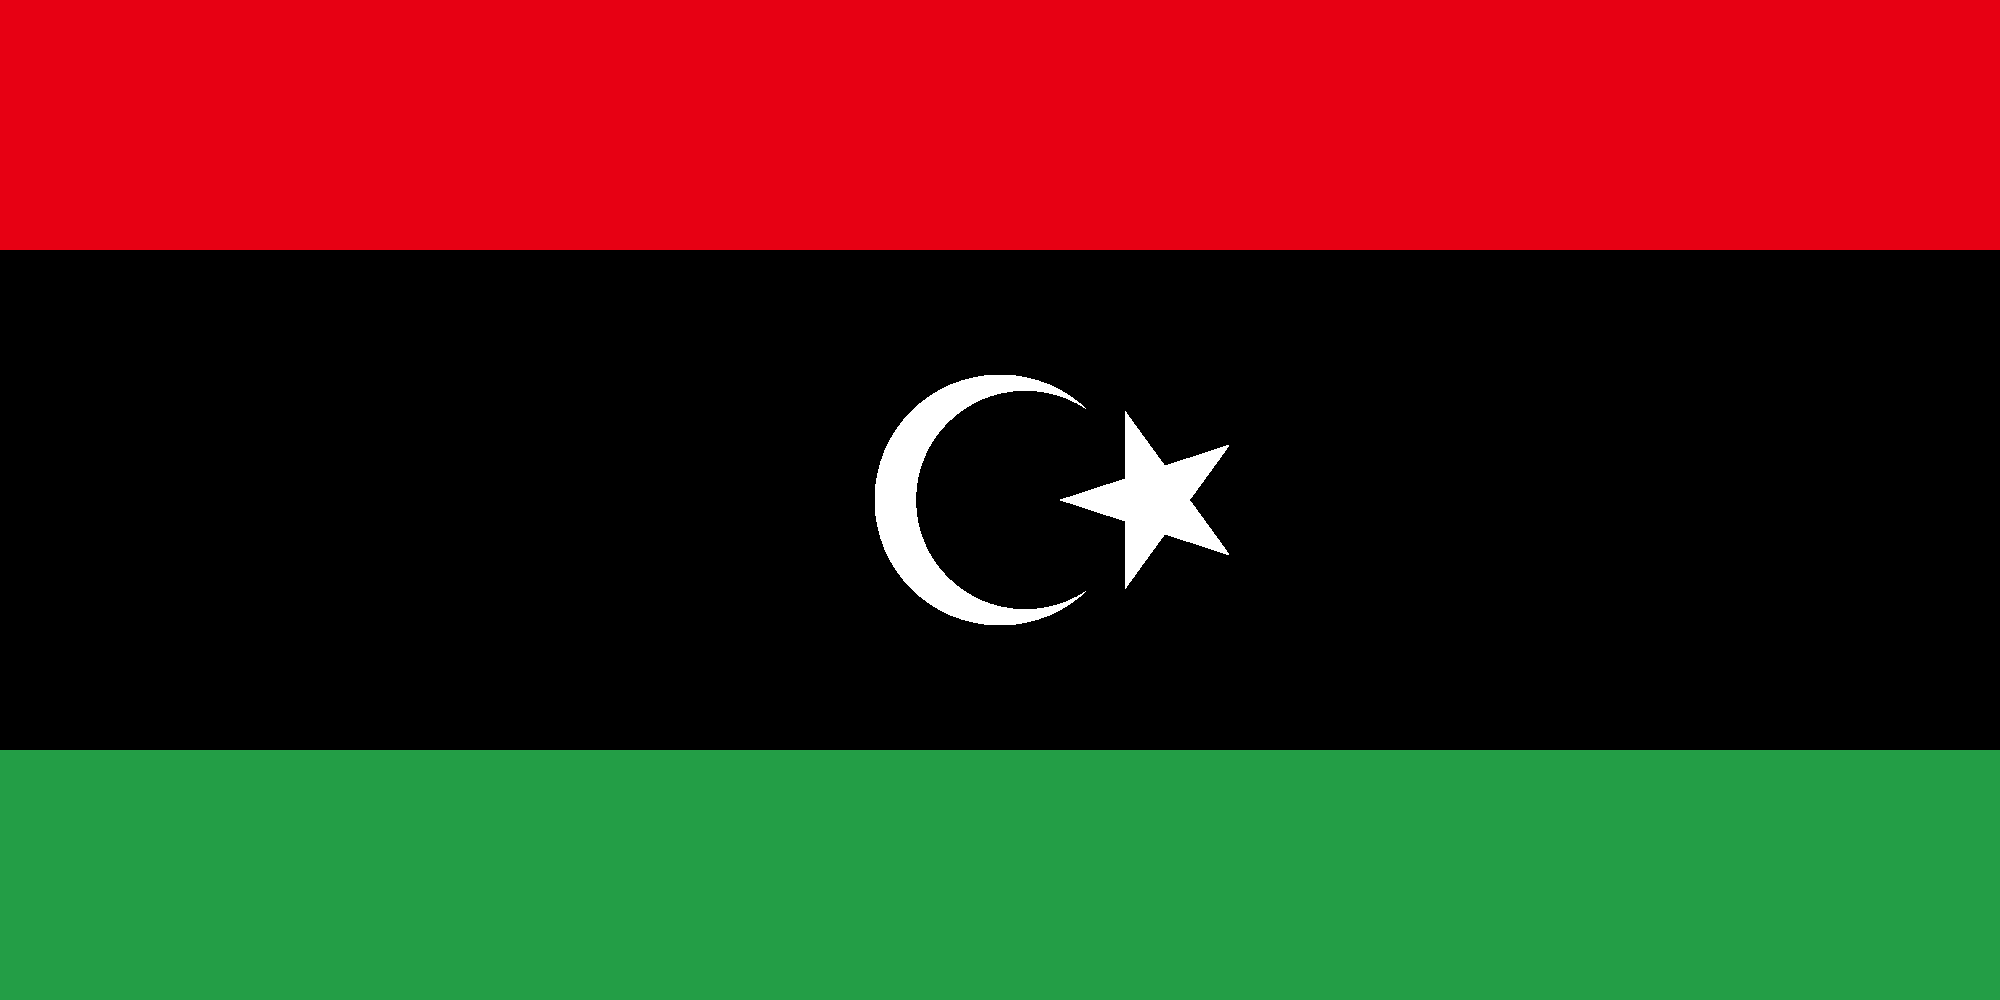
\includegraphics[height=0.66cm]{pdf/ly.pdf}\fontsize{22}{1}\selectfont\textbf{\  LIBYA \textcolor{myblue}{GENDER LANDSCAPE}}}

\begin{wraptable}{r}{0pt}\begingroup\fontsize{8}{10}\selectfont

\begin{tabular}[t]{lcl}

\textbf{Compared to:} & \textbf{Base Year} & \textbf{Region}\\
\midrule
>10\% Higher Value & 
\includegraphics[width=0.1in, height=0.1in]{upicon.png} & \cellcolor[HTML]{21908C}{}\\
Equal/No Change & 
\includegraphics[width=0.1in, height=0.1in]{righticon.png} & \cellcolor[HTML]{34608D}{}\\
>10\% Lower Value & 
\includegraphics[width=0.1in, height=0.1in]{downicon.png} & \cellcolor[HTML]{482576}{}\\
No Data & 
\includegraphics[width=0.1in, height=0.1in]{naicon.png} & \cellcolor{gray}{}\\

\end{tabular}
\endgroup{}\end{wraptable}

\begin{minipage}[t][1.7cm][t]{12cm}
\fontsize{9}{8}\selectfont\raggedright
This briefing showcases the gender landscape in Libya on key indicators helpful for monitoring gender equality and designing effective policy interventions. Gender equality fosters productivity gains, minimizes losses in wealth, reduces poverty, boosts shared prosperity, and supports green, resilient, and inclusive development. Libya is a Fragile, Conflict, or Violence (FCV) impacted country in medium-intensity conflict. 


\includegraphics[width=10pt]{pointer.png} Click the measures below to explore the \underline{\href{https://genderdata.worldbank.org/}{World Bank Gender Data Portal}}.
\end{minipage}
\vspace{6pt}
\vspace{16pt}

\begingroup\fontsize{7.5}{9.5}\selectfont

\begin{ThreePartTable}
\begin{TableNotes}[para]
\item \textit{Note: } 
\item \textcolor{darkgray}{The Middle East and North Africa (MNA)  region includes 21 countries (all income levels), as classified by The World Bank Group. Libya is an upper middle income (UMC) country, which includes 55 countries with a Gross National Income (GNI) per capita from \$4,096 to \$12,695 (calculated using the World Bank Atlas method). Data and definitions can be found on the \underline{\href{https://genderdata.worldbank.org/}{Gender Data Portal}}.} 

\textcolor{darkgray}{Country Baseline provides a reference from 1990 to 2010. Latest Value shows the latest available comparison from 2011 onwards. The arrow icon represents country increases or decreases over 10 percent relative to the base year. Peer comparisons show how Libya performs relative to the region, income group, and the world. Lighter and darker shades represent values 10 percent above and below regional peer values, respectively.}
\end{TableNotes}
\begin{longtable}[t]{>{\raggedright\arraybackslash}p{9cm}>{\raggedright\arraybackslash}p{1.1cm}>{}c>{}c>{}c>{}c>{}c>{}c>{}c>{}c}
\toprule
\multicolumn{2}{c}{\textbf{ }} & \multicolumn{5}{c}{\textbf{Country Performance}} & \multicolumn{3}{c}{\textbf{Peer Comparison}} \\
\cmidrule(l{3pt}r{3pt}){3-7} \cmidrule(l{3pt}r{3pt}){8-10}
\multicolumn{2}{c}{\textbf{ }} & \multicolumn{2}{c}{\textbf{Baseline}} & \multicolumn{1}{c}{\textbf{ }} & \multicolumn{2}{c}{\textbf{Latest}} & \multicolumn{3}{c}{\textbf{Latest}} \\
\cmidrule(l{3pt}r{3pt}){3-4} \cmidrule(l{3pt}r{3pt}){6-7} \cmidrule(l{3pt}r{3pt}){8-10}
\textbf{\textbf{}} & \textbf{\textbf{}} & \textbf{\textbf{Value}} & \textbf{\textbf{Year}} & \textbf{\textbf{}} & \textbf{\textbf{Value}} & \textbf{\textbf{Year}} & \textbf{\textbf{MNA}} & \textbf{\textbf{UMC}} & \textbf{\textbf{World}}\\
\midrule
\endfirsthead
\multicolumn{10}{@{}l}{\textit{(continued)}}\\
\toprule
\textbf{\textbf{}} & \textbf{\textbf{}} & \textbf{\textbf{Value}} & \textbf{\textbf{Year}} & \textbf{\textbf{}} & \textbf{\textbf{Value}} & \textbf{\textbf{Year}} & \textbf{\textbf{MNA}} & \textbf{\textbf{UMC}} & \textbf{\textbf{World}}\\
\midrule
\endhead

\endfoot
\bottomrule
\insertTableNotes
\endlastfoot
\addlinespace[0.3em]
\multicolumn{10}{l}{\cellcolor{lightgray}{\textbf{HUMAN ENDOWMENTS}}}\\
 & Female & \textcolor{gray}{NA} & \textcolor{gray}{NA} & 
\includegraphics[width=0.1in, height=0.1in]{naicon.png} & \cellcolor{gray}{\textcolor{white}{\textbf{NA}}} & \textcolor{gray}{NA} & \textcolor{gray}{NA} & \textcolor{gray}{NA} & \textcolor{gray}{NA}\\
\nopagebreak
\multirow{-2}{9cm}{\raggedright\arraybackslash \href{https://genderdata.worldbank.org/indicators/hd-hci-lays}{Learning-Adjusted Years of Schooling}} & Male & \textcolor{gray}{NA} & \textcolor{gray}{NA} & 
\includegraphics[width=0.1in, height=0.1in]{naicon.png} & \cellcolor{gray}{\textcolor{white}{\textbf{NA}}} & \textcolor{gray}{NA} & \textcolor{gray}{NA} & \textcolor{gray}{NA} & \textcolor{gray}{NA}\\
\cmidrule{1-10}\pagebreak[0]
 & Female & \textcolor[HTML]{000004}{77.8} & \textcolor[HTML]{000004}{2004} & 
\includegraphics[width=0.1in, height=0.1in]{naicon.png} & \cellcolor{gray}{\textcolor{white}{\textbf{NA}}} & \textcolor{gray}{NA} & \textcolor[HTML]{000004}{73.2} & \textcolor{gray}{NA} & \textcolor[HTML]{000004}{83.3}\\
\nopagebreak
\multirow{-2}{9cm}{\raggedright\arraybackslash \href{https://genderdata.worldbank.org/indicators/se-adt}{Literacy rate (\% 15+)}} & Male & \textcolor[HTML]{000004}{93.8} & \textcolor[HTML]{000004}{2004} & 
\includegraphics[width=0.1in, height=0.1in]{naicon.png} & \cellcolor{gray}{\textcolor{white}{\textbf{NA}}} & \textcolor{gray}{NA} & \textcolor[HTML]{000004}{85.6} & \textcolor{gray}{NA} & \textcolor[HTML]{000004}{90.1}\\
\cmidrule{1-10}\pagebreak[0]
 & Female & \textcolor{gray}{NA} & \textcolor{gray}{NA} & 
\includegraphics[width=0.1in, height=0.1in]{naicon.png} & \cellcolor{gray}{\textcolor{white}{\textbf{NA}}} & \textcolor{gray}{NA} & \textcolor[HTML]{000004}{91.8} & \textcolor{gray}{NA} & \textcolor[HTML]{000004}{89.9}\\
\nopagebreak
\multirow{-2}{9cm}{\raggedright\arraybackslash \href{https://genderdata.worldbank.org/indicators/se-prm-cmpt-zs}{Primary completion rate (\% of relevant group)}} & Male & \textcolor{gray}{NA} & \textcolor{gray}{NA} & 
\includegraphics[width=0.1in, height=0.1in]{naicon.png} & \cellcolor{gray}{\textcolor{white}{\textbf{NA}}} & \textcolor{gray}{NA} & \textcolor[HTML]{000004}{94.9} & \textcolor{gray}{NA} & \textcolor[HTML]{000004}{90.3}\\
\cmidrule{1-10}\pagebreak[0]
\href{https://genderdata.worldbank.org/indicators/sp-dyn-tfrt-in}{Fertility rate, total (births per woman)} &  & \textcolor[HTML]{000004}{2.48} & \textcolor[HTML]{000004}{2010} & 
\includegraphics[width=0.1in, height=0.1in]{downicon.png} & \cellcolor[HTML]{482576}{\textcolor{white}{\textbf{2.17}}} & \textcolor[HTML]{000004}{2020} & \textcolor[HTML]{000004}{2.74} & \textcolor{gray}{NA} & \textcolor[HTML]{000004}{2.39}\\
\cmidrule{1-10}\pagebreak[0]
\href{https://genderdata.worldbank.org/indicators/sp-ado-tfrt}{Adolescent fertility rate (births per 1,000 women 15-19)} &  & \textcolor[HTML]{000004}{6.18} & \textcolor[HTML]{000004}{2010} & 
\includegraphics[width=0.1in, height=0.1in]{downicon.png} & \cellcolor[HTML]{482576}{\textcolor{white}{\textbf{5.61}}} & \textcolor[HTML]{000004}{2020} & \textcolor[HTML]{000004}{39.0} & \textcolor{gray}{NA} & \textcolor[HTML]{000004}{41.0}\\
\cmidrule{1-10}\pagebreak[0]
\href{https://genderdata.worldbank.org/indicators/sh-sta-brtc-zs}{Births attended by skilled health staff (\% of total)} &  & \textcolor{gray}{NA} & \textcolor{gray}{NA} & 
\includegraphics[width=0.1in, height=0.1in]{naicon.png} & \cellcolor{gray}{\textcolor{white}{\textbf{NA}}} & \textcolor{gray}{NA} & \textcolor{gray}{NA} & \textcolor{gray}{NA} & \textcolor{gray}{NA}\\
\cmidrule{1-10}\pagebreak[0]
 & Female & \textcolor[HTML]{000004}{17.3} & \textcolor[HTML]{000004}{2010} & 
\includegraphics[width=0.1in, height=0.1in]{righticon.png} & \cellcolor[HTML]{355F8D}{\textcolor{white}{\textbf{17.6}}} & \textcolor[HTML]{000004}{2019} & \textcolor[HTML]{000004}{17.4} & \textcolor{gray}{NA} & \textcolor[HTML]{000004}{14.8}\\
\nopagebreak
\multirow{-2}{9cm}{\raggedright\arraybackslash \href{https://genderdata.worldbank.org/indicators/sh-dyn-ncom-zs}{Mortality from chronic vascular disease, cancer, diabetes or cardiorespiratory disease between 30 and 70 (\%)}} & Male & \textcolor[HTML]{000004}{18.3} & \textcolor[HTML]{000004}{2010} & 
\includegraphics[width=0.1in, height=0.1in]{righticon.png} & \cellcolor[HTML]{482576}{\textcolor{white}{\textbf{19.7}}} & \textcolor[HTML]{000004}{2019} & \textcolor[HTML]{000004}{22.9} & \textcolor{gray}{NA} & \textcolor[HTML]{000004}{21.7}\\
\cmidrule{1-10}\pagebreak[0]
 & Female & \textcolor[HTML]{000004}{0.10} & \textcolor[HTML]{000004}{2010} & 
\includegraphics[width=0.1in, height=0.1in]{righticon.png} & \cellcolor[HTML]{355F8D}{\textcolor{white}{\textbf{0.10}}} & \textcolor[HTML]{000004}{2020} & \textcolor[HTML]{000004}{0.10} & \textcolor{gray}{NA} & \textcolor[HTML]{000004}{0.40}\\
\nopagebreak
\multirow{-2}{9cm}{\raggedright\arraybackslash \href{https://genderdata.worldbank.org/indicators/sh-hiv-1524-zs}{Prevalence of HIV (\% 15-24)}} & Male & \textcolor[HTML]{000004}{0.10} & \textcolor[HTML]{000004}{2010} & 
\includegraphics[width=0.1in, height=0.1in]{righticon.png} & \cellcolor[HTML]{355F8D}{\textcolor{white}{\textbf{0.10}}} & \textcolor[HTML]{000004}{2020} & \textcolor[HTML]{000004}{0.10} & \textcolor{gray}{NA} & \textcolor[HTML]{000004}{0.20}\\
\cmidrule{1-10}\pagebreak[0]
\addlinespace[0.3em]
\multicolumn{10}{l}{\cellcolor{lightgray}{\textbf{ECONOMIC OPPORTUNITY}}}\\
 & Female & \textcolor[HTML]{000004}{33.9} & \textcolor[HTML]{000004}{2010} & 
\includegraphics[width=0.1in, height=0.1in]{righticon.png} & \cellcolor[HTML]{21908C}{\textcolor{white}{\textbf{34.1}}} & \textcolor[HTML]{000004}{2021} & \textcolor[HTML]{000004}{18.6} & \textcolor{gray}{NA} & \textcolor[HTML]{000004}{46.3}\\
\nopagebreak
\multirow{-2}{9cm}{\raggedright\arraybackslash \href{https://genderdata.worldbank.org/indicators/sl-tlf-acti-zs}{Labor force participation rate (\% 15+, modeled ILO estimate)}} & Male & \textcolor[HTML]{000004}{61.3} & \textcolor[HTML]{000004}{2010} & 
\includegraphics[width=0.1in, height=0.1in]{righticon.png} & \cellcolor[HTML]{482576}{\textcolor{white}{\textbf{61.0}}} & \textcolor[HTML]{000004}{2021} & \textcolor[HTML]{000004}{70.0} & \textcolor{gray}{NA} & \textcolor[HTML]{000004}{71.7}\\
\cmidrule{1-10}\pagebreak[0]
 & Female & \textcolor[HTML]{000004}{66.7} & \textcolor[HTML]{000004}{2010} & 
\includegraphics[width=0.1in, height=0.1in]{righticon.png} & \cellcolor[HTML]{482576}{\textcolor{white}{\textbf{64.7}}} & \textcolor[HTML]{000004}{2019} & \textcolor[HTML]{000004}{73.8} & \textcolor{gray}{NA} & \textcolor[HTML]{000004}{54.6}\\
\nopagebreak
\multirow{-2}{9cm}{\raggedright\arraybackslash \href{https://genderdata.worldbank.org/indicators/sl-emp-work-zs}{Wage and salaried workers (\% of employment, modeled ILO estimate)}} & Male & \textcolor[HTML]{000004}{66.5} & \textcolor[HTML]{000004}{2010} & 
\includegraphics[width=0.1in, height=0.1in]{downicon.png} & \cellcolor[HTML]{482576}{\textcolor{white}{\textbf{60.2}}} & \textcolor[HTML]{000004}{2019} & \textcolor[HTML]{000004}{69.8} & \textcolor{gray}{NA} & \textcolor[HTML]{000004}{53.0}\\
\cmidrule{1-10}\pagebreak[0]
 & Female & \textcolor[HTML]{000004}{23.5} & \textcolor[HTML]{000004}{2010} & 
\includegraphics[width=0.1in, height=0.1in]{downicon.png} & \cellcolor[HTML]{355F8D}{\textcolor{white}{\textbf{15.9}}} & \textcolor[HTML]{000004}{2019} & \textcolor[HTML]{000004}{15.7} & \textcolor{gray}{NA} & \textcolor[HTML]{000004}{25.3}\\
\nopagebreak
\multirow{-2}{9cm}{\raggedright\arraybackslash \href{https://genderdata.worldbank.org/indicators/sl-empl-zs}{Employment in agriculture (\% of employment, modeled ILO estimate)}} & Male & \textcolor[HTML]{000004}{19.2} & \textcolor[HTML]{000004}{2010} & 
\includegraphics[width=0.1in, height=0.1in]{downicon.png} & \cellcolor[HTML]{21908C}{\textcolor{white}{\textbf{16.6}}} & \textcolor[HTML]{000004}{2019} & \textcolor[HTML]{000004}{14.4} & \textcolor{gray}{NA} & \textcolor[HTML]{000004}{27.6}\\
\cmidrule{1-10}\pagebreak[0]
 & Female & \textcolor{gray}{NA} & \textcolor{gray}{NA} & 
\includegraphics[width=0.1in, height=0.1in]{naicon.png} & \cellcolor{gray}{\textcolor{white}{\textbf{NA}}} & \textcolor{gray}{NA} & \textcolor[HTML]{000004}{43.9} & \textcolor{gray}{NA} & \textcolor{gray}{NA}\\
\nopagebreak
\multirow{-2}{9cm}{\raggedright\arraybackslash \href{https://genderdata.worldbank.org/indicators/sl-uem-neet-zs}{Share of youth not in education, employment or training (\% of youth population)}} & Male & \textcolor{gray}{NA} & \textcolor{gray}{NA} & 
\includegraphics[width=0.1in, height=0.1in]{naicon.png} & \cellcolor{gray}{\textcolor{white}{\textbf{NA}}} & \textcolor{gray}{NA} & \textcolor[HTML]{000004}{17.0} & \textcolor{gray}{NA} & \textcolor{gray}{NA}\\
\cmidrule{1-10}\pagebreak[0]
\href{https://genderdata.worldbank.org/indicators/sp-pop-dpnd}{Age dependency ratio (\% of working-age population)} &  & \textcolor[HTML]{000004}{49.1} & \textcolor[HTML]{000004}{2010} & 
\includegraphics[width=0.1in, height=0.1in]{righticon.png} & \cellcolor[HTML]{482576}{\textcolor{white}{\textbf{47.7}}} & \textcolor[HTML]{000004}{2020} & \textcolor[HTML]{000004}{55.5} & \textcolor{gray}{NA} & \textcolor[HTML]{000004}{54.6}\\
\cmidrule{1-10}\pagebreak[0]
 & Female & \textcolor{gray}{NA} & \textcolor{gray}{NA} & 
\includegraphics[width=0.1in, height=0.1in]{naicon.png} & \cellcolor{gray}{\textcolor{white}{\textbf{59.6}}} & \textcolor[HTML]{000004}{2017} & \textcolor{gray}{NA} & \textcolor[HTML]{000004}{69.0} & \textcolor[HTML]{000004}{63.7}\\
\nopagebreak
\multirow{-2}{9cm}{\raggedright\arraybackslash \href{https://genderdata.worldbank.org/indicators/fin1-t-a}{Financial institution account (\% 15+)}} & Male & \textcolor{gray}{NA} & \textcolor{gray}{NA} & 
\includegraphics[width=0.1in, height=0.1in]{naicon.png} & \cellcolor{gray}{\textcolor{white}{\textbf{70.7}}} & \textcolor[HTML]{000004}{2017} & \textcolor{gray}{NA} & \textcolor[HTML]{000004}{76.6} & \textcolor[HTML]{000004}{70.6}\\
\cmidrule{1-10}\pagebreak[0]
 & Female & \textcolor{gray}{NA} & \textcolor{gray}{NA} & 
\includegraphics[width=0.1in, height=0.1in]{naicon.png} & \cellcolor{gray}{\textcolor{white}{\textbf{4.90}}} & \textcolor[HTML]{000004}{2017} & \textcolor{gray}{NA} & \textcolor[HTML]{000004}{4.29} & \textcolor[HTML]{000004}{5.26}\\
\nopagebreak
\multirow{-2}{9cm}{\raggedright\arraybackslash \href{https://genderdata.worldbank.org/indicators/fin21-t-a}{Borrowed to start, operate, or expand a farm or business (\% 15+)}} & Male & \textcolor{gray}{NA} & \textcolor{gray}{NA} & 
\includegraphics[width=0.1in, height=0.1in]{naicon.png} & \cellcolor{gray}{\textcolor{white}{\textbf{13.5}}} & \textcolor[HTML]{000004}{2017} & \textcolor{gray}{NA} & \textcolor[HTML]{000004}{6.78} & \textcolor[HTML]{000004}{7.57}\\
\cmidrule{1-10}\pagebreak[0]
\href{https://genderdata.worldbank.org/indicators/ic-frm-femo-zs}{Firms with female participation in ownership (\% of firms)} &  & \textcolor{gray}{NA} & \textcolor{gray}{NA} & 
\includegraphics[width=0.1in, height=0.1in]{naicon.png} & \cellcolor{gray}{\textcolor{white}{\textbf{NA}}} & \textcolor{gray}{NA} & \textcolor[HTML]{000004}{19.0} & \textcolor{gray}{NA} & \textcolor[HTML]{000004}{33.1}\\
\cmidrule{1-10}\pagebreak[0]
\addlinespace[0.3em]
\multicolumn{10}{l}{\cellcolor{lightgray}{\textbf{VOICE AND AGENCY}}}\\
\href{https://genderdata.worldbank.org/indicators/ic-frm-femm-zs}{Firms with female top manager (\% of firms)} &  & \textcolor{gray}{NA} & \textcolor{gray}{NA} & 
\includegraphics[width=0.1in, height=0.1in]{naicon.png} & \cellcolor{gray}{\textcolor{white}{\textbf{NA}}} & \textcolor{gray}{NA} & \textcolor[HTML]{000004}{6.50} & \textcolor{gray}{NA} & \textcolor[HTML]{000004}{17.8}\\
\cmidrule{1-10}\pagebreak[0]
\href{https://genderdata.worldbank.org/indicators/sg-gen-parl-zs}{Proportion of seats held by women in national parliaments (\%)} &  & \textcolor[HTML]{000004}{7.69} & \textcolor[HTML]{000004}{2010} & 
\includegraphics[width=0.1in, height=0.1in]{upicon.png} & \cellcolor[HTML]{355F8D}{\textcolor{white}{\textbf{16.0}}} & \textcolor[HTML]{000004}{2021} & \textcolor[HTML]{000004}{17.0} & \textcolor{gray}{NA} & \textcolor[HTML]{000004}{26.1}\\
\cmidrule{1-10}\pagebreak[0]
\href{https://genderdata.worldbank.org/indicators/sp-2024-fe-zs}{Women who were first married by 18 (\% of women 20-24)} &  & \textcolor{gray}{NA} & \textcolor{gray}{NA} & 
\includegraphics[width=0.1in, height=0.1in]{naicon.png} & \cellcolor{gray}{\textcolor{white}{\textbf{NA}}} & \textcolor{gray}{NA} & \textcolor{gray}{NA} & \textcolor{gray}{NA} & \textcolor{gray}{NA}\\
\cmidrule{1-10}\pagebreak[0]
\href{https://genderdata.worldbank.org/indicators/sg-vaw-1549-zs}{Proportion of women subjected to physical and/or sexual violence in the last 12 months (\% of ever-partnered women 15-49)} &  & \textcolor{gray}{NA} & \textcolor{gray}{NA} & 
\includegraphics[width=0.1in, height=0.1in]{naicon.png} & \cellcolor{gray}{\textcolor{white}{\textbf{NA}}} & \textcolor{gray}{NA} & \textcolor{gray}{NA} & \textcolor{gray}{NA} & \textcolor{gray}{NA}\\*
\end{longtable}
\end{ThreePartTable}
\endgroup{}

\newpage
\clearpage

\raggedright
\vspace{.2cm}
\fcolorbox{white}{white}{\color{black}
\begin{minipage}[c][1.7cm][t]{19.5cm}
\begin{minipage}[c][1.7cm][t]{6cm}
\begin{spacing}{2}\fontsize{14}{1}\selectfont   
Women, Business and the Law in Libya
\normalsize
\end{spacing}\end{minipage}\hspace{0.5cm}
\begin{minipage}[c][1.7cm][t]{12.75cm}
\fontsize{9}{8}\selectfont   
\textbf{\underline{\href{https://wbl.worldbank.org/en/wbl}{Women, Business and the Law (WBL) 2022}}} presents an index covering 190 economies, structured around the life cycle of a working woman. In total, 35 questions are scored across eight indicators. \textbf{Libya scores 50 out of 100,} while the regional average across Middle East and North Africa is 80.
\normalsize
\end{minipage}
\end{minipage}}

\centering
\begin{minipage}[c][4.2cm][t]{2.1cm}\begin{mybox}\centering
\vspace{.3cm}

\includegraphics[height=.75cm]{overall.png}

\vspace{.3cm}
\fontsize{7.5}{1}\selectfont   
\textbf{\underline{\href{https://genderdata.worldbank.org/indicators/sg-law-indx}{Overall}}}\normalsize 

\vspace{18pt}
\fontsize{14}{1}\selectfont 
\centering\circled{\href{https://genderdata.worldbank.org/indicators/sg-law-indx}{50}}
\vspace{.3cm}
\normalsize\end{mybox}\end{minipage}
\begin{minipage}[c][4.2cm][t]{2.1cm}\begin{mybox}\centering
\vspace{.3cm}

\includegraphics[height=.75cm]{mobility.png}

\vspace{.3cm}
\fontsize{7.5}{1}\selectfont   
\textbf{\underline{\href{https://genderdata.worldbank.org/indicators/sg-law-indx-mo}{Mobility}}}\normalsize 

\vspace{16pt}
\fontsize{14}{1}\selectfont 
\centering\circled{\href{https://genderdata.worldbank.org/indicators/sg-law-indx-mo}{75}}
\vspace{.3cm}
\normalsize\end{mybox}\end{minipage}
\begin{minipage}[c][4.2cm][t]{2.1cm}\begin{mybox}\centering
\vspace{.3cm}

\includegraphics[height=.75cm]{workplace.png}

\vspace{.3cm}
\fontsize{7.5}{1}\selectfont   
\textbf{\underline{\href{https://genderdata.worldbank.org/indicators/sg-law-indx-wp}{Workplace}}}\normalsize 

\vspace{16pt}
\fontsize{14}{1}\selectfont 
\centering\circled{\href{https://genderdata.worldbank.org/indicators/sg-law-indx-wp}{50}}
\vspace{.3cm}
\normalsize\end{mybox}\end{minipage}
\begin{minipage}[c][4.2cm][t]{2.1cm}\begin{mybox}\centering
\vspace{.3cm}

\includegraphics[height=.75cm]{pay.png}

\vspace{.3cm}
\fontsize{7.5}{1}\selectfont   
\textbf{\underline{\href{https://genderdata.worldbank.org/indicators/sg-law-indx-py}{Pay}}}\normalsize 

\vspace{16pt}
\fontsize{14}{1}\selectfont 
\centering\circled{\href{https://genderdata.worldbank.org/indicators/sg-law-indx-py}{75}}
\vspace{.3cm}
\normalsize\end{mybox}\end{minipage}
\begin{minipage}[c][4.2cm][t]{2.1cm}\begin{mybox}\centering
\vspace{.3cm}

\includegraphics[height=.75cm]{marriage.png}

\vspace{.3cm}
\fontsize{7.5}{1}\selectfont   
\textbf{\underline{\href{https://genderdata.worldbank.org/indicators/sg-law-indx-mr}{Marriage}}}\normalsize 

\vspace{16pt}
\fontsize{14}{1}\selectfont 
\centering\circled{{\href{https://genderdata.worldbank.org/indicators/sg-law-indx-mr}{20}}}
\vspace{.3cm}
\normalsize\end{mybox}\end{minipage}
\begin{minipage}[c][4.2cm][t]{2.1cm}\begin{mybox}\centering
\vspace{.3cm}

\includegraphics[height=.75cm]{parenthood.png}

\vspace{.3cm}
\fontsize{7.5}{1}\selectfont   
\textbf{\underline{\href{https://genderdata.worldbank.org/indicators/sg-law-indx-pr}{Parent-}}}
\textbf{\underline{\href{https://genderdata.worldbank.org/indicators/sg-law-indx-pr}{hood}}}\normalsize 

\vspace{8.5pt}
\fontsize{14}{1}\selectfont 
\centering\circled{{\href{https://genderdata.worldbank.org/indicators/sg-law-indx-pr}{40}}}

\vspace{.3cm}
\normalsize\end{mybox}\end{minipage}
\begin{minipage}[c][4.2cm][t]{2.1cm}\begin{mybox}\centering

\vspace{.3cm}

\includegraphics[height=.75cm]{entrepreneur.png}

\vspace{.3cm}
\fontsize{7.5}{1}\selectfont   
\textbf{\underline{\href{https://genderdata.worldbank.org/indicators/sg-law-indx-en}{Entrepre-}}}
\textbf{\underline{\href{https://genderdata.worldbank.org/indicators/sg-law-indx-en}{neurship}}}\normalsize 

\vspace{6pt}
\fontsize{15}{1}\selectfont 

\centering\circled{{\href{https://genderdata.worldbank.org/indicators/sg-law-indx-en}{75}}}
\vspace{.3cm}
\normalsize\end{mybox}\end{minipage}
\begin{minipage}[c][4.2cm][t]{2.1cm}\begin{mybox}\centering
\vspace{.3cm}

\includegraphics[height=.75cm]{assets.png}

\vspace{.45cm}
\fontsize{7.5}{1}\selectfont   
\textbf{\underline{\href{https://genderdata.worldbank.org/indicators/sg-law-indx-as}{Assets}}}
  
\normalsize 
\vspace{17pt}
\fontsize{14}{1}\selectfont 
\centering\circled{{\href{https://genderdata.worldbank.org/indicators/sg-law-indx-as}{40}}}

\vspace{.3cm}
\normalsize\end{mybox}\end{minipage}
\begin{minipage}[c][4.2cm][t]{2.1cm}\begin{mybox}\centering

\vspace{.3cm}

\includegraphics[height=.75cm]{pension.png}

\vspace{.3cm}
\fontsize{7.5}{1}\selectfont   
\textbf{\underline{\href{https://genderdata.worldbank.org/indicators/sg-law-indx-pe}{Pension}}}\normalsize 

\vspace{18pt}
\fontsize{14}{1}\selectfont 
\centering\circled{{\href{https://genderdata.worldbank.org/indicators/sg-law-indx-pe}{25}}}

\vspace{.3cm}
\normalsize\end{mybox}\end{minipage}

\vspace{.3cm}

\centering\rule{19.5cm}{0.5pt}

\vspace{.3cm}

\begin{minipage}[c][1.65cm][t]{19.5cm}
\begin{minipage}[c][1.65cm][t]{6cm}
\begin{spacing}{2}\fontsize{14}{1}\selectfont   
A Closer Look at Gender Equality in Libya
\normalsize
\end{spacing}\end{minipage}\hspace{0.5cm}
\begin{minipage}[c][1.65cm][t]{12.75cm}
\fontsize{9}{8}\selectfont   
Despite some progress, gender gaps, gender-based violence, and disadvantageous social norms facing women and girls persist, and gains in human capital of women and girls remain untapped. Turning human capital investments into economic gains means addressing multiple barriers to women’s economic empowerment, including improving their voice and agency.
\normalsize
\end{minipage}
\end{minipage}

\vspace{.15cm}

\begin{minipage}[t][4.7cm][t]{19.5cm}
\href{https://genderdata.worldbank.org/indicators/hd-hci-ovrl}{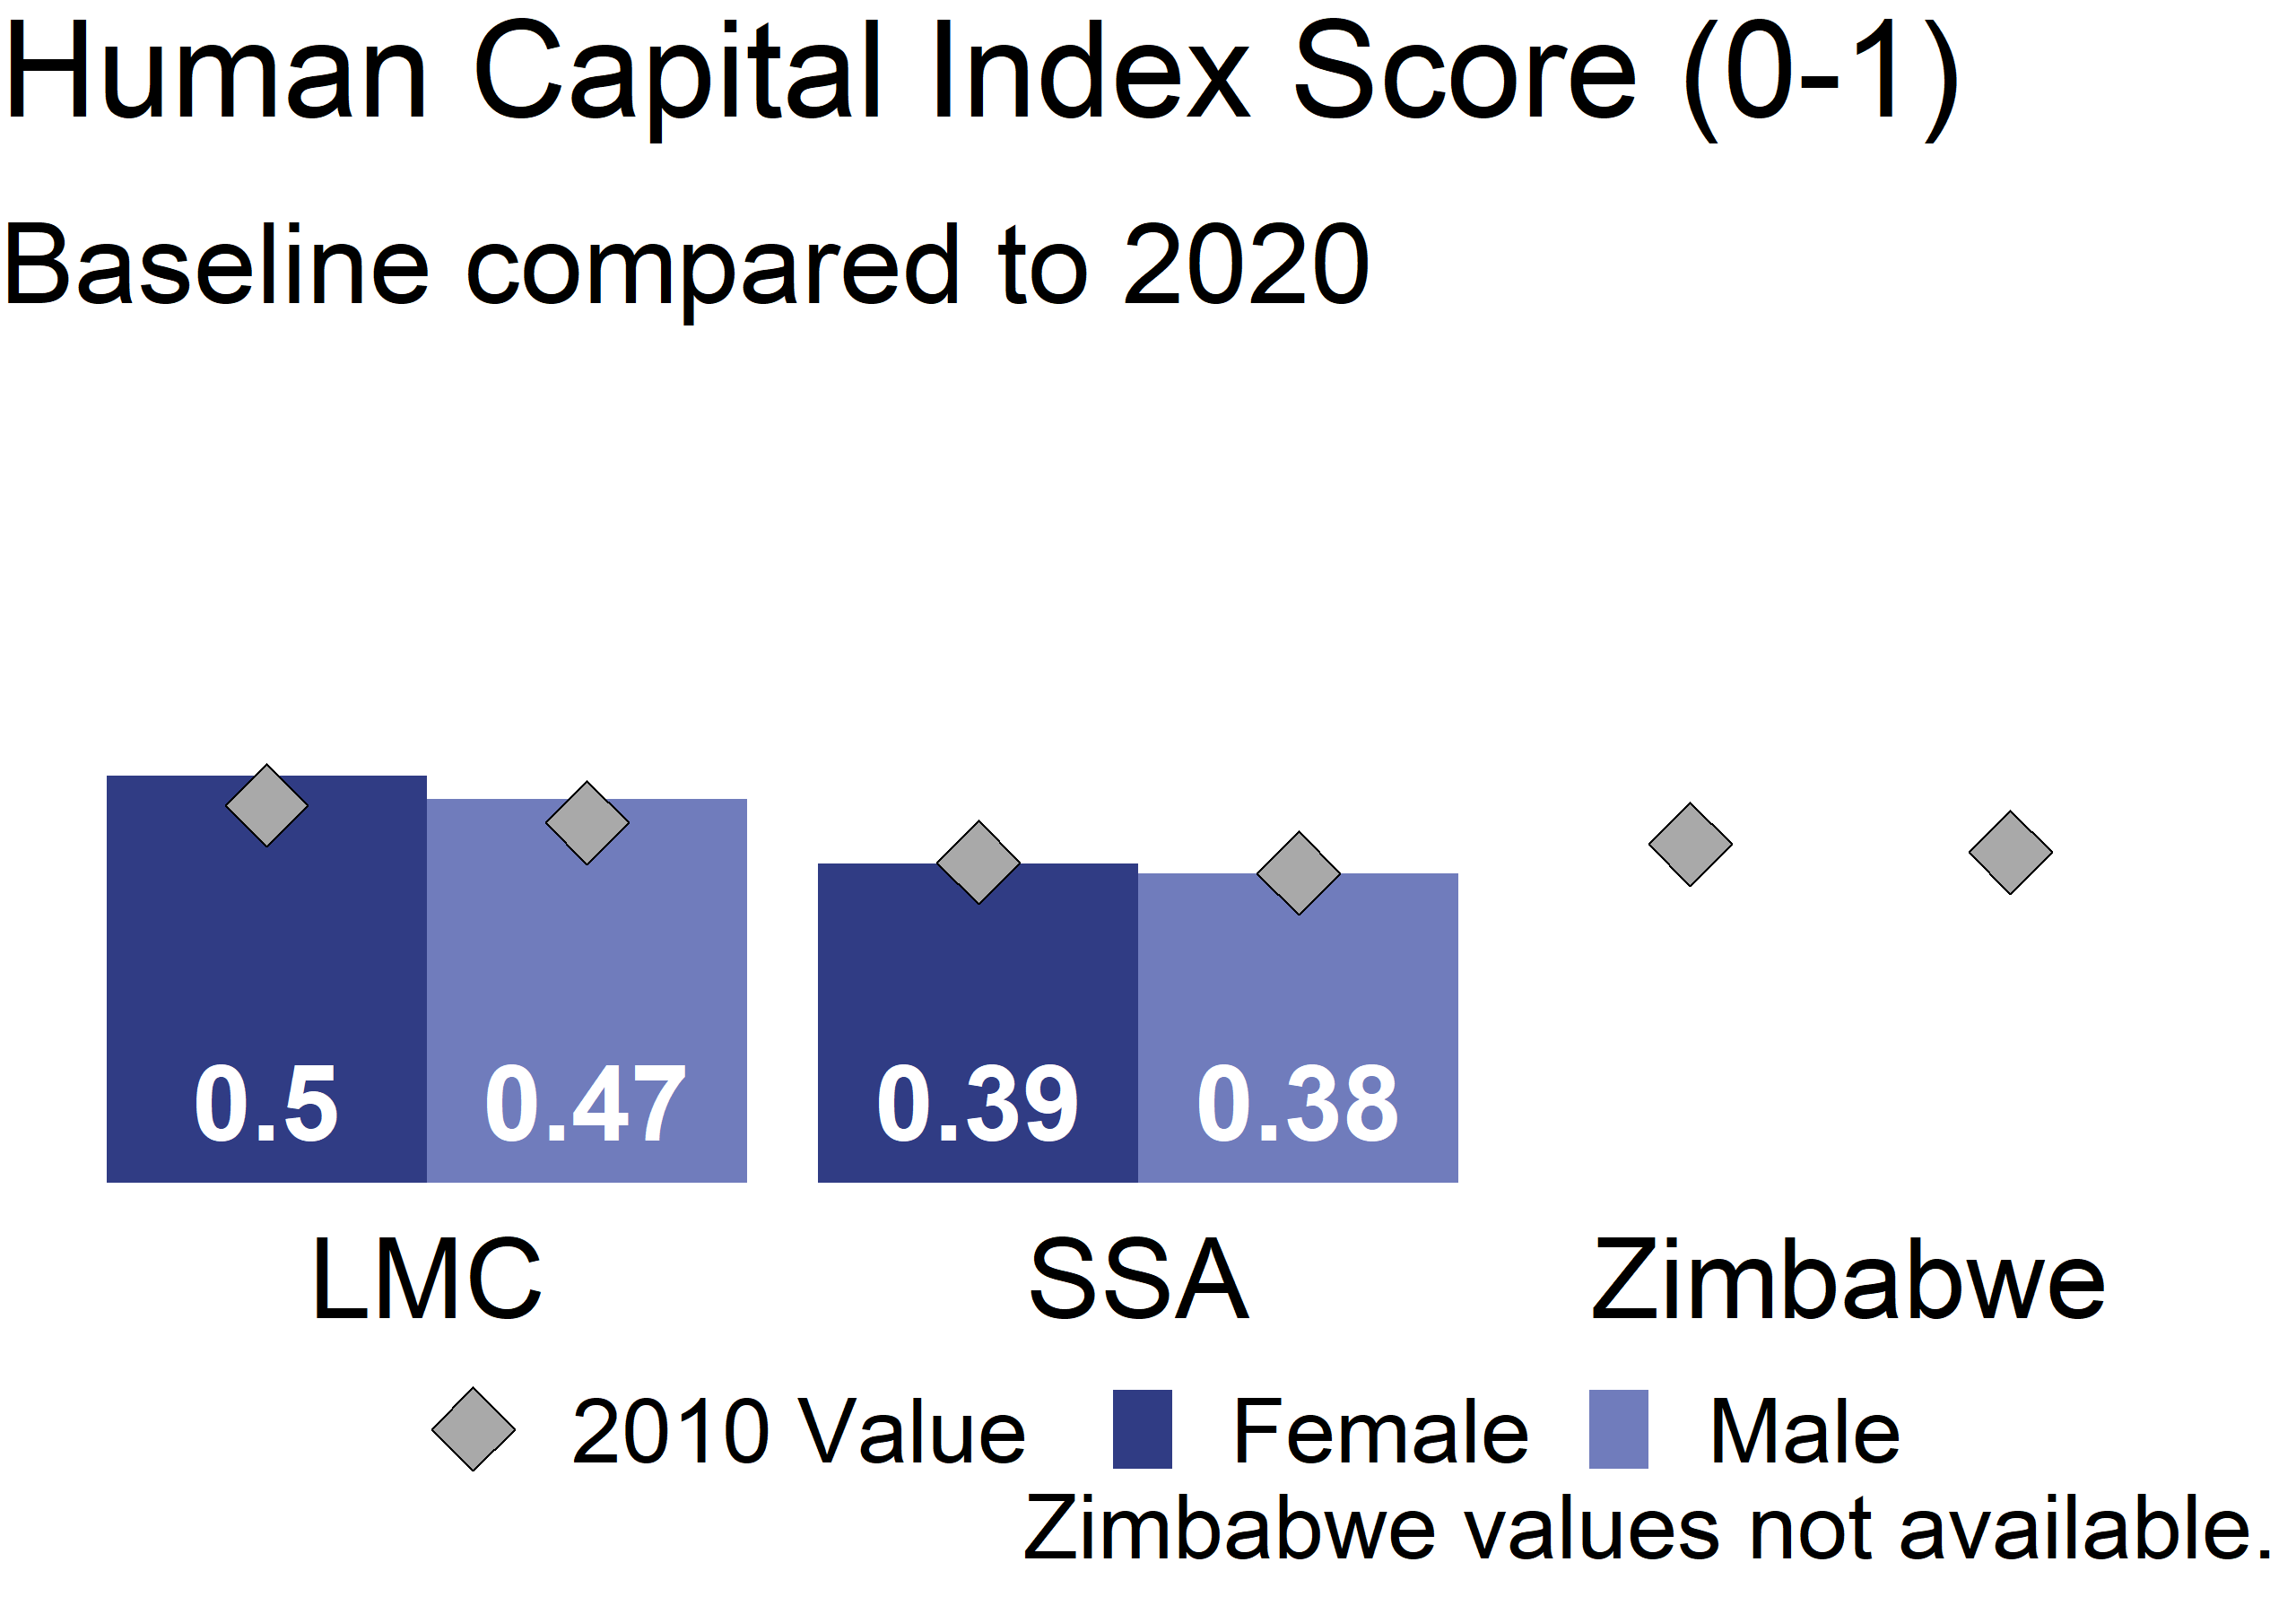
\includegraphics[height=4.7cm]{HCIplot.png}}\hspace{.2cm}
\href{https://genderdata.worldbank.org/indicators/sl-tlf-acti-zs/}{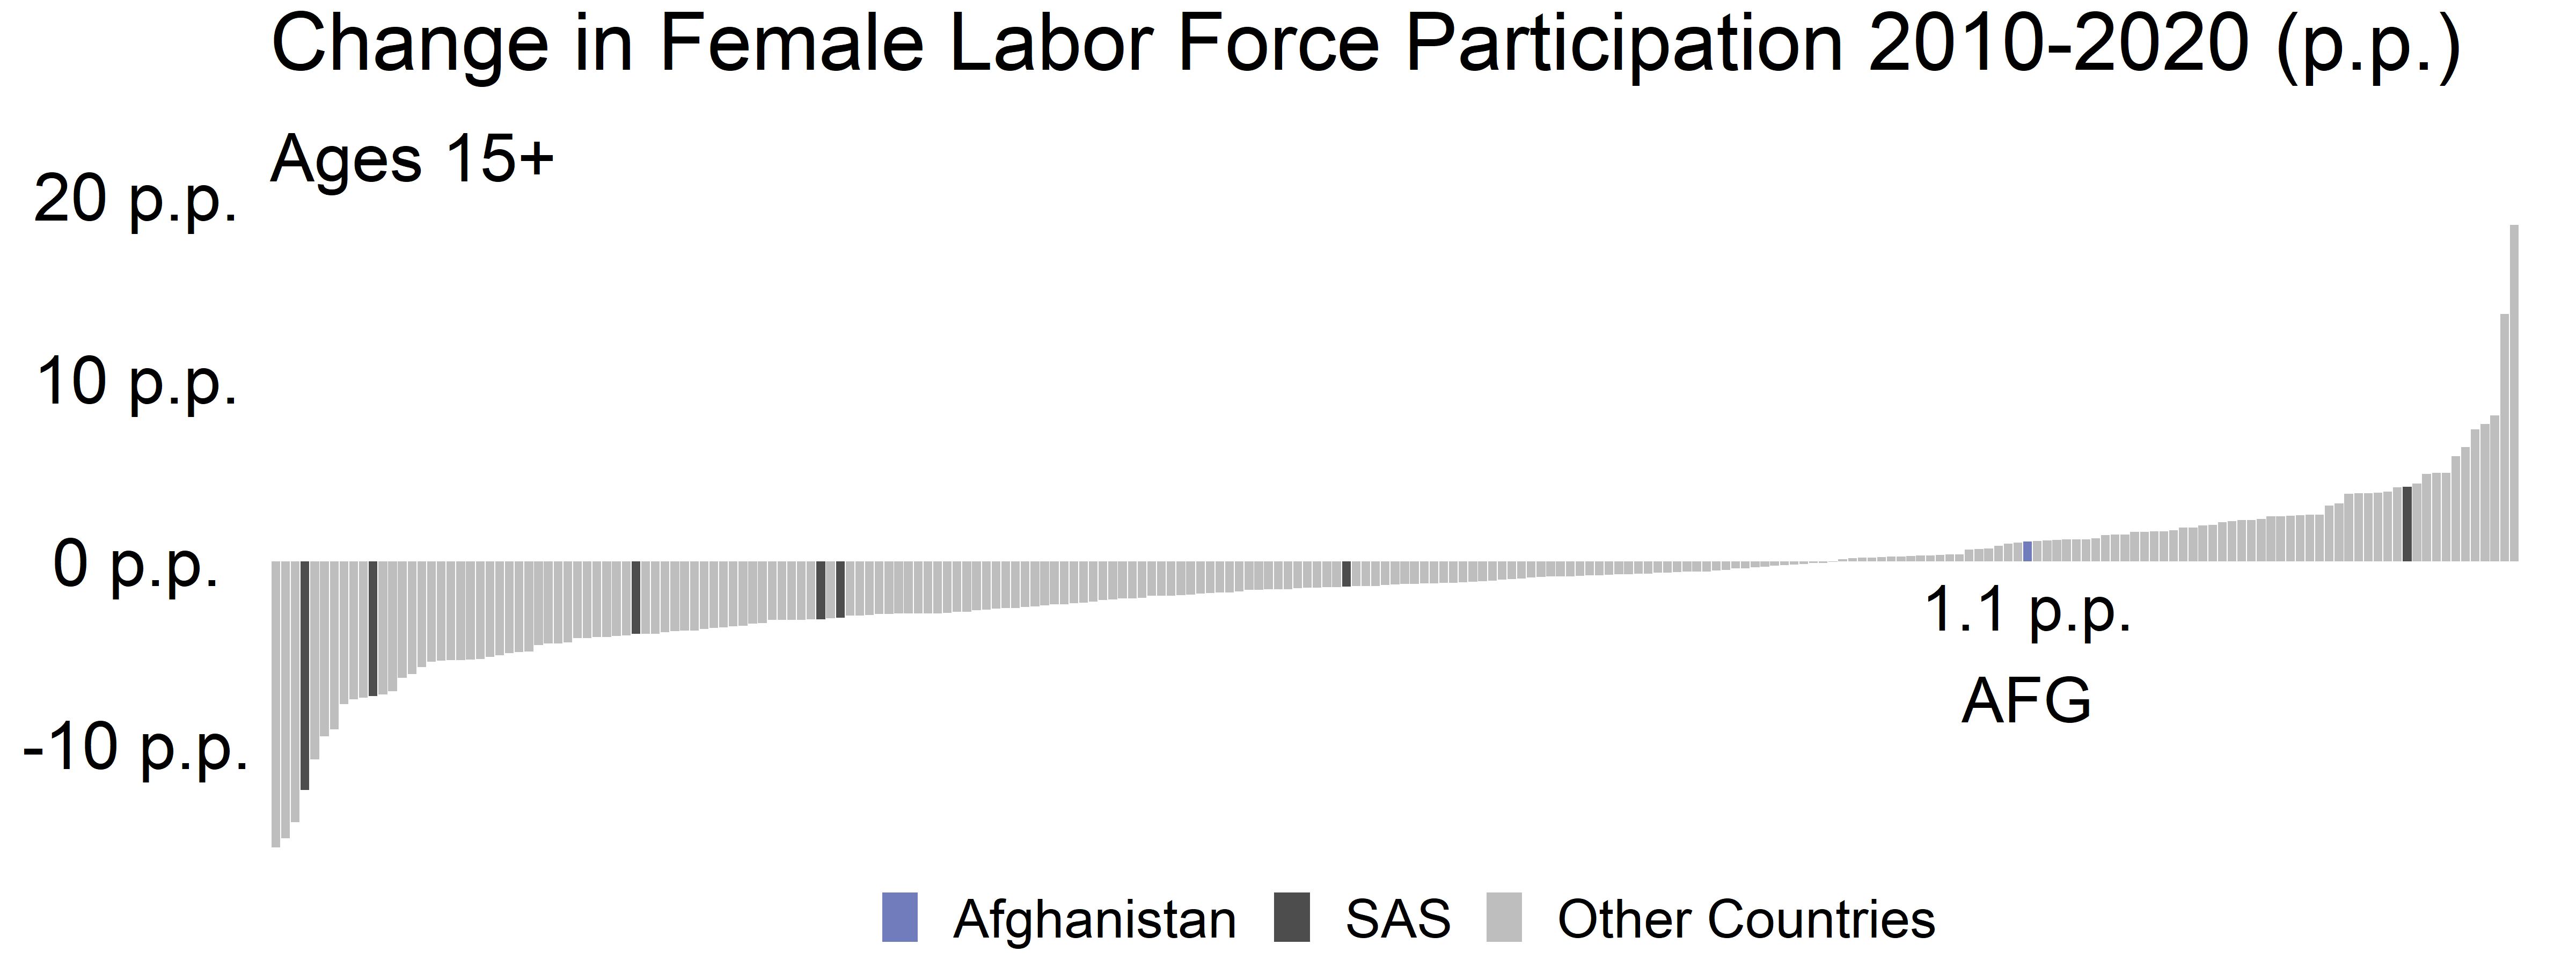
\includegraphics[height=4.7cm]{LFPplot.png}}  
\end{minipage}

\vspace{.2cm}

\centering\fontsize{10}{8}\selectfont

------ \textbf{Unpacking the Numbers in Libya} ------ \normalsize

\fboxrule.6pt\fcolorbox{white}{white}{\color{black}
\begin{minipage}[c][3.3cm][t]{3.15cm}
\vspace{.15cm}\fontsize{10}{5}\centering
\textbf{11 percent}

\centering\rule{2.5cm}{0.5pt}
\vspace{.15cm}

\fontsize{9}{5}\selectfont
11 percent more men than women in Libya have an account at a financial institution 
\textbf{\underline{\href{https://genderdata.worldbank.org/indicators/fin1-t-a}{(2017)}}}
\normalsize\end{minipage}}\hspace{0.45cm}\fboxrule.6pt\fcolorbox{white}{white}{\color{black}
\begin{minipage}[c][3.3cm][t]{3.15cm}
\vspace{.15cm}\fontsize{10}{5}\centering
\textbf{27 points}

\centering\rule{2.5cm}{0.5pt}
\vspace{.15cm}


\fontsize{9}{5}\selectfont
Men and women have a 27 percentage point gap in labor force participation 
\textbf{\underline{\href{27 points}{(2021)}}}
\normalsize\end{minipage}}\hspace{0.45cm}
\fboxrule.6pt\fcolorbox{white}{white}{\color{black}
\begin{minipage}[c][3.3cm][t]{3.15cm}
\vspace{.15cm}\fontsize{10}{5}\centering
\textbf{40 percent}

\centering\rule{2.5cm}{0.5pt}
\vspace{.15cm}

\fontsize{9}{5}\selectfont
40 percent of married women ages 15 to 49 report not having access to contraceptives 
\textbf{\underline{\href{https://genderdata.worldbank.org/indicators/sp-uwt-tfrt}{(2014)}}}
\normalsize\end{minipage}}\hspace{0.45cm}
\fboxrule.6pt\fcolorbox{white}{white}{\color{black}
\begin{minipage}[c][3.3cm][t]{3.15cm}
\vspace{.15cm}\fontsize{10}{5}\centering
\textbf{5.2 times}

\centering\rule{2.5cm}{0.5pt}
\vspace{.15cm}

\fontsize{9}{5}\selectfont
Men hold 5.2 times as many seats in the national parliament as women 
\textbf{\underline{\href{https://genderdata.worldbank.org/indicators/sg-gen-parl-zs}{(2021)}}}
\normalsize\end{minipage}}\hspace{0.45cm}
\fboxrule.6pt\fcolorbox{white}{white}{\color{black}
\begin{minipage}[c][3.3cm][t]{3.15cm}
\vspace{.15cm}\fontsize{10}{5}\centering

\textbf{0.97 times}

\centering\rule{2.5cm}{0.5pt}
\vspace{.15cm}

\fontsize{9}{5}\selectfont
A man is 0.97 times as likely to have used the internet to pay bills or to buy something online in the past year
\textbf{\underline{\href{https://genderdata.worldbank.org/indicators/fin14abca-t-d}{(2017)}}}
\normalsize\end{minipage}}

\vspace{.15cm}

\centering\rule{19.5cm}{0.5pt}

\vspace{0.15cm}

\fcolorbox{white}{white}{\color{black}
\raggedright\begin{minipage}[t][5cm][t]{9cm}
\fontsize{10}{12}\selectfont
\textbf{ LEARN MORE}
\fontsize{9}{12}\selectfont

\begin{itemize}
  \item[]\textbf{\underline{\href{https://www.worldbank.org/en/topic/gender}{The World Bank in Gender}}}: This portal features the latest research, news, and events around gender equality in international development.

  \item[]\textbf{\underline{\href{https://wbl.worldbank.org/en/wbl}{Women, Business and the Law}}}: This portal includes reports, data, and  news on the laws and regulations that affect women's economic opportunity.
  
  \item[]\textbf{\underline{\href{https://openknowledge.worldbank.org/handle/10986/23425}{World Bank Group Gender Strategy (FY16-FY23)}}}: This 2015 report outlines the World Bank Group's strategy to promote gender equality.
\end{itemize}

\end{minipage}}
\fcolorbox{white}{white}{\color{black}
\raggedright\begin{minipage}[t][5cm][t]{9cm}
\fontsize{10}{12}\selectfont
\textbf{ }
\fontsize{9}{12}\selectfont

\begin{itemize}
  \item[]\textbf{\underline{\href{https://genderdata.worldbank.org/}{World Bank Gender Data Portal}}}: This open data tool shares the latest statistics and research to improve understanding and inform policy choices.
  
  \item[]\textbf{\underline{\href{https://www.worldbank.org/en/programs/mena-gender-innovation-lab}{MENA Gender Innovation Lab}}}: This page features policy research by the GIL, evaluating innovative solutions to close priority gender gaps in the region.
  
  \item[]\textbf{\underline{\href{}{}}}
\end{itemize}

\end{minipage}}

\end{document}
